\appendix

% \chapter{\label{appendixpingo}Hints for PINGO user}
% 
% Some {\CDO} operators have the same name as in PINGO but
% the meaning is different.
% The following table gives an overview of those operators.
% 
% \vspace{2mm}
% \begin{tabular}[c]{|l||l|l|}
% \hline
% Operator name  & {\CDO}                   & PINGO \\
% \hline
% \hline
% min            & Minimum of two fields  & Time minimum \\
% \hline
% max            & Maximum of two fields  & Time maximum \\
% \hline
% daymean        & Daily mean             & Multi-year daily mean \\
% \hline
% daymin         & Daily minimum          & Multi-year daily minimum \\
% \hline
% daymax         & Daily maximum          & Multi-year daily maximum \\
% \hline
% monmean        & Monthly mean           & Multi-year monthly mean \\
% \hline
% monmin         & Monthly minimum        & Multi-year monthly minimum \\
% \hline
% monmax         & Monthly maximum        & Multi-year monthly maximum \\
% \hline
% seasmean       & Seasonally mean        & Multi-year seasonally mean \\
% \hline
% \end{tabular}
% \vspace{2mm}
% 
% There are also some {\CDO} operators with the same functionality
% as in PINGO but the name is different.
% The following table gives an overview of those operators.
% 
% \vspace{2mm}
% \begin{tabular}[c]{|l||l|l|}
% \hline
%                              & {\CDO}       & PINGO \\
% \hline
% \hline
% Maximum of two fields        & max        & max2 \\
% \hline
% Minimum of two fields        & min        & min2 \\
% \hline
% Field mean, min, max         & fldmean, fldmin, fldmax    & meanr minr, maxr\\
% \hline
% Time mean, min, max          & timmean, timmin, timmax    & mean, min, max \\
% \hline
% Daily mean, min, max         & daymean, daymin, daymax    & daymeans, daymins, daymaxs \\
% \hline
% Monthly mean, min, max       & monmean, monmin, monmax    & monmeans, monmins, monmaxs \\
% \hline
% Yearly mean, min, max        & yearmean, yearmin, yearmax   & yearmeans, yearmins, yearmaxs \\
% \hline
% Running mean                 & runmean    & runmeans \\
% \hline
% Seasonally mean              & seasmean   & seasmeans \\
% \hline
% Multi-year daily mean        & ydaymean   & daymean  \\
% \hline
% Multi-year monthly mean      & ymonmean   & monmean  \\
% \hline
% Multi-year seasonally mean   & yseasmean  & seasmean  \\
% \hline
% \end{tabular}
% \vspace{2mm}



\chapter{\label{environment}Environment Variables}

The following table describes the environment variables that affect {\CDO}.

\begin{tabular}[t]{|>{\columncolor{pcolor1}}l|r|l|}
\hline
\rowcolor{pcolor2}
%\cellcolor{pcolor2}
{\bf Variable name}           &  {\bf Default} & {\bf Description} \\ \hline
CDO\_FILE\_SUFFIX             &   None   &  Default file suffix. This suffix will be added to the output file \\
                                           &               &  name instead of the filename extension derived from the file \\
                                           &               & format. NULL will disable the adding of a file suffix. \\ \hline
CDO\_HISTORY\_INFO        &         1   & Append netCDF global attribute histroy \\ \hline
CDO\_PCTL\_NBINS            &     101    & Number of histogram bins. \\ \hline
CDO\_RESET\_HISTORY       &         0  & Set to 1 to reset the netCDF {\it history} global attribute.\\ \hline
CDO\_REMAP\_NORM         &  fracarea & Choose the normalization for the conservative interpolation \\
CDO\_REMAP\_RADIUS       &  180       & Remap search radius in degree. Used by the operators \\
                                                     &        & remapdis and remapnn. \\ \hline
CDO\_TIMESTAT\_DATE     &  None   & Set the date information of a time statistic operator to \\
                                           &             &  the "first", "middle" or "last" contributing timestep.\\ \hline
CDO\_USE\_FFTW               &         1  & Set to 0 to switch off usage of FFTW. Used in the Filter module.\\ \hline
CDO\_VERSION\_INFO        &         1  & Set to 0 to disable netCDF global attribute CDO \\ \hline
\end{tabular}


\chapter{\label{openmp}Parallelized operators}

Some of the {\CDO} operators are parallelized with OpenMP.
To use {\CDO} with multiple OpenMP threads, you have to set the number of threads with the option '-P'.
Here is an example to distribute the bilinear interpolation on 8 OpenMP threads:
\begin{lstlisting}[frame=single, backgroundcolor=\color{pcolor2}, basicstyle=\ttfamily, columns=flexible]
   cdo -P 8  remapbil,targetgrid  ifile  ofile
\end{lstlisting}
The following {\CDO} operators are parallelized with OpenMP:

\begin{tabular}[t]{|l|>{\columncolor{pcolor1}}l|l|}
\hline
\rowcolor{pcolor2}
%\cellcolor{pcolor2}
{\bf Module}     &  {\bf Operator} & {\bf Description} \\ \hline
Detrend      & detrend         & Detrend \\ \hline
Ensstat      & ensmin          & Ensemble minimum \\ \hline
Ensstat      & ensmax          & Ensemble maximum \\ \hline
Ensstat      & enssum          & Ensemble sum \\ \hline
Ensstat      & ensmean         & Ensemble mean \\ \hline
Ensstat      & ensavg          & Ensemble average \\ \hline
Ensstat      & ensvar          & Ensemble variance \\ \hline
Ensstat      & ensstd          & Ensemble standard deviation \\ \hline
Ensstat      & enspctl         & Ensemble percentiles \\ \hline
Filter        & bandpass       &  Bandpass filtering \\ \hline
Filter        & lowpass        &  Lowpass filtering \\ \hline
Filter        & highpass      &   Highpass filtering \\ \hline
Fourier      & fourier         & Fourier transformation \\ \hline
Genweights   & genbil          & Generate bilinear interpolation weights \\ \hline
Genweights   & genbic          & Generate bicubic interpolation weights \\ \hline
Genweights   & gendis          & Generate distance-weighted average remap weights \\ \hline
Genweights   & gennn           & Generate nearest neighbor remap weights \\ \hline
Genweights   & gencon          & Generate 1st order conservative remap weights \\ \hline
Genweights   & gencon2         & Generate 2nd order conservative remap weights \\ \hline
Genweights   & genlaf          & Generate largest area fraction remap weights \\ \hline
Gridboxstat  & gridboxmin      & Gridbox minimum \\ \hline
Gridboxstat  & gridboxmax      & Gridbox maximum \\ \hline
Gridboxstat  & gridboxsum      & Gridbox sum \\ \hline
Gridboxstat  & gridboxmean     & Gridbox mean \\ \hline
Gridboxstat  & gridboxavg      & Gridbox average \\ \hline
Gridboxstat  & gridboxvar      & Gridbox variance \\ \hline
Gridboxstat  & gridboxstd      & Gridbox standard deviation \\ \hline
Remapeta     & remapeta        & Remap vertical hybrid level \\ \hline
Remap        & remapbil        & Bilinear interpolation \\ \hline
Remap        & remapbic        & Bicubic interpolation \\ \hline
Remap        & remapdis        & Distance-weighted average remapping \\ \hline
Remap        & remapnn         & Nearest neighbor remapping \\ \hline
Remap        & remapcon        & First order conservative remapping \\ \hline
Remap        & remapcon2       & Second order conservative remapping \\ \hline
Remap        & remaplaf        & Largest area fraction remapping \\ \hline

\end{tabular}



\chapter{\label{stdnametable}Standard name table}

The following CF standard names are supported by {\CDO}.

\begin{tabular}[t]{|>{\columncolor{pcolor1}}l|r|r|l|}
\hline
\rowcolor{pcolor2}
%\cellcolor{pcolor2}
{\bf CF standard name}       &  Units & {\bf GRIB 1 code} & {\bf variable name} \\ \hline
surface\_geopotential           &  m2 s-2 &  129   &  geosp \\ \hline
air\_temperature                    & K           & 130  &  ta \\ \hline
specific\_humidity                 & 1           & 133  & hus  \\ \hline
surface\_air\_pressure           & Pa          & 134  & aps  \\ \hline
air\_pressure\_at\_sea\_level & Pa         & 151  & psl  \\ \hline
geopotential\_height              & m         & 156  &  zg \\ \hline
\end{tabular}


\chapter{\label{appendixgrid}Grid description examples}

\section{Example of a curvilinear grid description}
Here is an example for the {\CDO} description of a curvilinear grid.
xvals/yvals describe the positions of the 6x5 quadrilateral grid cells.
The first 4 values of xbounds/ybounds are the corners of the first grid cell.
\lstset{moredelim=**[is][\color{red}]{|}{|}}
\begin{lstlisting}[frame=single, backgroundcolor=\color{pcolor1}, basicstyle=\footnotesize]
gridtype  = curvilinear
gridsize  = 30
xsize     = 6
ysize     = 5
xvals     =  |-21|  -11    0   11   21   30  -25  -13    0   13
              25   36  -31  -16    0   16   31   43  -38  -21
               0   21   38   52  -51  -30    0   30   51   64
xbounds   =  |-23  -14  -17  -28|       -14   -5   -6  -17        -5    5    6   -6
               5   14   17    6        14   23   28   17        23   32   38   28
             -28  -17  -21  -34       -17   -6   -7  -21        -6    6    7   -7
               6   17   21    7        17   28   34   21        28   38   44   34
             -34  -21  -27  -41       -21   -7   -9  -27        -7    7    9   -9
               7   21   27    9        21   34   41   27        34   44   52   41
             -41  -27  -35  -51       -27   -9  -13  -35        -9    9   13  -13
               9   27   35   13        27   41   51   35        41   52   63   51
             -51  -35  -51  -67       -35  -13  -21  -51       -13   13   21  -21
              13   35   51   21        35   51   67   51        51   63   77   67
yvals     =   |29|   32   32   32   29   26   39   42   42   42
              39   35   48   51   52   51   48   43   57   61
              62   61   57   51   65   70   72   70   65   58
ybounds   =   |23   26   36   32|        26   27   37   36        27   27   37   37
              27   26   36   37        26   23   32   36        23   19   28   32
              32   36   45   41        36   37   47   45        37   37   47   47
              37   36   45   47        36   32   41   45        32   28   36   41
              41   45   55   50        45   47   57   55        47   47   57   57
              47   45   55   57        45   41   50   55        41   36   44   50
              50   55   64   58        55   57   67   64        57   57   67   67
              57   55   64   67        55   50   58   64        50   44   51   58
              58   64   72   64        64   67   77   72        67   67   77   77
              67   64   72   77        64   58   64   72        58   51   56   64
\end{lstlisting}

\begin{figure}[b]
\ifpdfoutput{
{\scalebox{0.99}{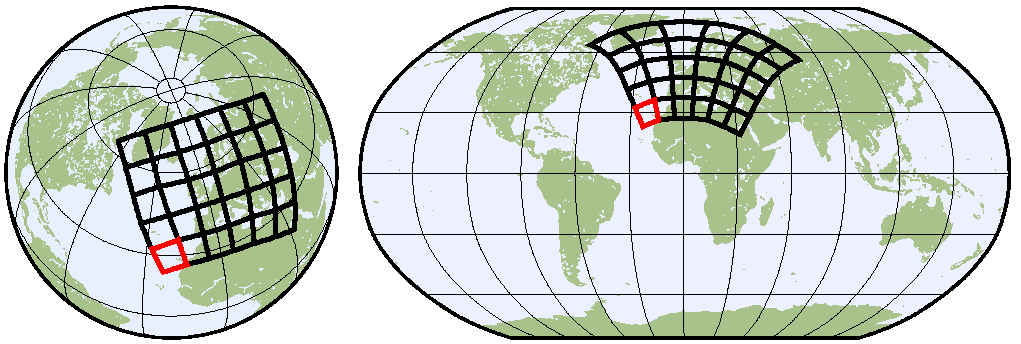
\includegraphics{grids/curv.pdf}}}
}{
{\scalebox{0.99}{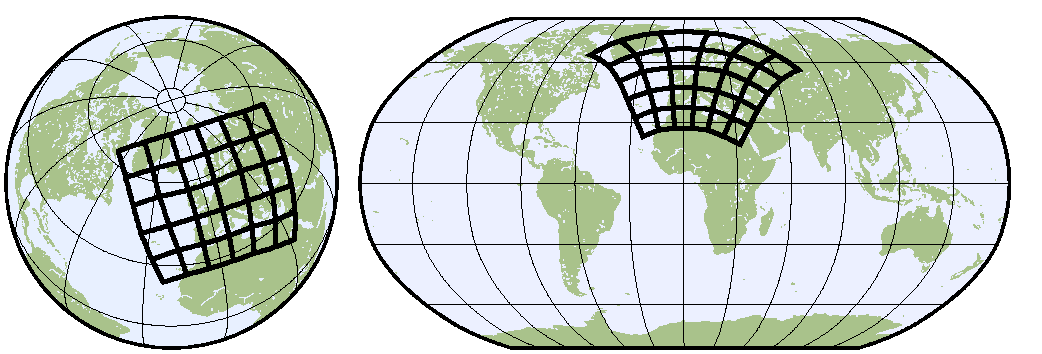
\includegraphics{grids/curv}}}
}
\caption[curvgrid]{Orthographic and Robinson projection of the
  curvilinear grid,  the first grid cell is colored red}
\end{figure}

\newpage
\section{Example description for an unstructured grid}
Here is an example of the {\CDO} description for an unstructured grid.
xvals/yvals describe the positions of 30 independent hexagonal grid cells.
The first 6 values of xbounds/ybounds are the corners of the first
grid cell.
The grid cell corners have to rotate counterclockwise.
The first grid cell is colored red.
\begin{lstlisting}[frame=single, backgroundcolor=\color{pcolor1}, basicstyle=\footnotesize]
gridtype  = unstructured
gridsize  = 30
nvertex   = 6
xvals     =  |-36|   36    0  -18   18  108   72   54   90  180  144  126  162 -108 -144 
            -162 -126  -72  -90  -54    0   72   36  144  108 -144  180  -72 -108  -36 
xbounds   =  |339    0    0  288  288  309|        21   51   72   72    0    0
               0   16   21    0  339  344       340    0   -0  344  324  324
              20   36   36   16    0    0        93  123  144  144   72   72
              72   88   93   72   51   56        52   72   72   56   36   36
              92  108  108   88   72   72       165  195  216  216  144  144
             144  160  165  144  123  128       124  144  144  128  108  108
             164  180  180  160  144  144       237  267  288  288  216  216
             216  232  237  216  195  200       196  216  216  200  180  180
             236  252  252  232  216  216       288  304  309  288  267  272
             268  288  288  272  252  252       308  324  324  304  288  288
             345  324  324   36   36   15        36   36  108  108   87   57
              20   15   36   57   52   36       108  108  180  180  159  129
              92   87  108  129  124  108       180  180  252  252  231  201
             164  159  180  201  196  180       252  252  324  324  303  273
             236  231  252  273  268  252       308  303  324  345  340  324
yvals     =   |58|   58   32    0    0   58   32    0    0   58   32    0    0   58   32 
               0    0   32    0    0  -58  -58  -32  -58  -32  -58  -32  -58  -32  -32 
ybounds   =   |41   53   71   71   53   41|        41   41   53   71   71   53
              11   19   41   53   41   19       -19   -7   11   19    7  -11
             -19  -11    7   19   11   -7        41   41   53   71   71   53
              11   19   41   53   41   19       -19   -7   11   19    7  -11
             -19  -11    7   19   11   -7        41   41   53   71   71   53
              11   19   41   53   41   19       -19   -7   11   19    7  -11
             -19  -11    7   19   11   -7        41   41   53   71   71   53
              11   19   41   53   41   19       -19   -7   11   19    7  -11
             -19  -11    7   19   11   -7        11   19   41   53   41   19
             -19   -7   11   19    7  -11       -19  -11    7   19   11   -7
             -41  -53  -71  -71  -53  -41       -53  -71  -71  -53  -41  -41
             -19  -41  -53  -41  -19  -11       -53  -71  -71  -53  -41  -41
             -19  -41  -53  -41  -19  -11       -53  -71  -71  -53  -41  -41
             -19  -41  -53  -41  -19  -11       -53  -71  -71  -53  -41  -41
             -19  -41  -53  -41  -19  -11       -19  -41  -53  -41  -19  -11
\end{lstlisting}

\begin{figure}[b]

\ifpdfoutput{
{\scalebox{1}{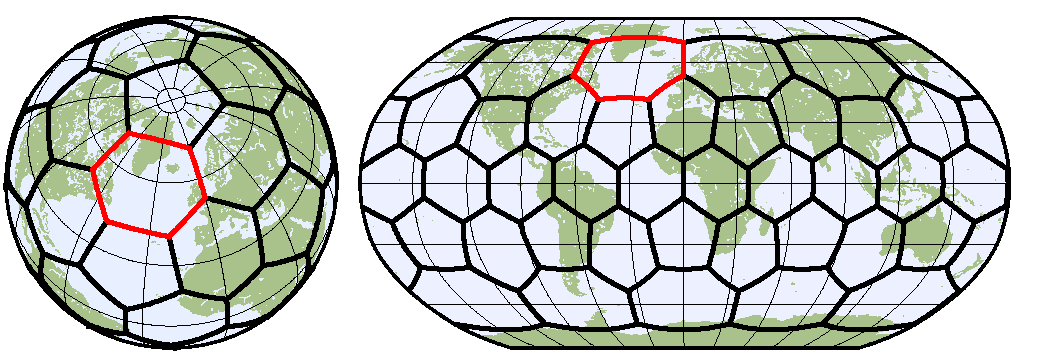
\includegraphics{grids/cell.pdf}}}
}{
{\scalebox{1}{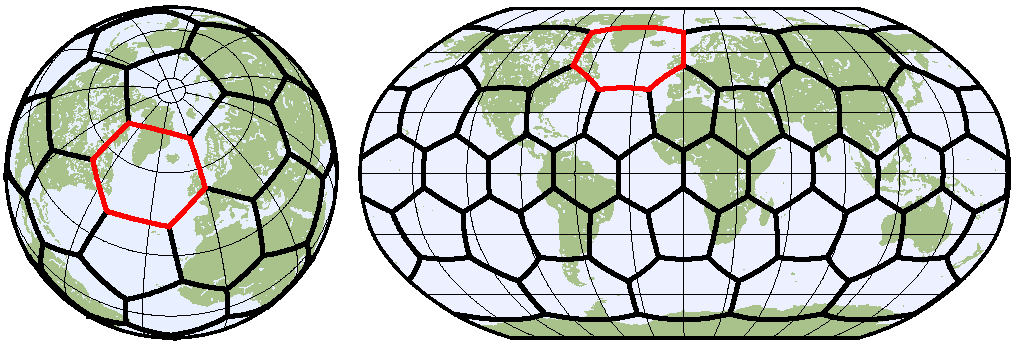
\includegraphics{grids/cell}}}
}
\caption[cellgrid]{Orthographic and Robinson projection of the unstructured grid}
\end{figure}

%%% Local Variables: 
%%% mode: latex
%%% TeX-master: "grid"
%%% End: 
